% Created 2022-09-19 Mon 17:05
% Intended LaTeX compiler: pdflatex
\documentclass[11pt]{article}
\usepackage[utf8]{inputenc}
\usepackage[T1]{fontenc}
\usepackage{graphicx}
\usepackage{grffile}
\usepackage[a4paper,margin=1in]{geometry}
\usepackage{longtable}
\usepackage{wrapfig}
\usepackage{rotating}
\usepackage[normalem]{ulem}
\usepackage{amsmath}
\usepackage{textcomp}
\usepackage{amssymb}
\usepackage{capt-of}
\usepackage{hyperref}
\usepackage{subcaption}
\author{Mridul Gupta}
\date{\today}
\title{}
\hypersetup{
 pdfauthor={Mridul Gupta},
 pdftitle={},
 pdfkeywords={},
 pdfsubject={},
 pdfcreator={Emacs 27.1 (Org mode 9.3)}, 
 pdflang={English}}
\begin{document}
% \section{First pass}

% At iteration \(k\) (crosscheck this),
% \begin{align*}
%     &P:\min_{\alpha\in\mathbb{R}}\;\phi(\alpha)\\
%     &\mbox{where }\phi(\alpha)=x_k-\alpha\nabla f(x)\lvert_{x=x_k}\\
%     &\\
%     &\mbox{and then}\\
%     &\\
%     &\hat{\alpha_k}=\underset{\alpha\in\mathbb{R}}{\operatorname{argmin}}\;\phi(\alpha)\\
%     &x_{k+1}=x_k-\hat{\alpha_k}\nabla f(x)\lvert_{x=x_k}
% \end{align*}
% \vspace{1cm}
% 
% How to do line search?
% 
% \begin{enumerate}
%     \item Start with a bracket.
%     \item How? Go forward and backward.
%     \item Once we have \([a,b]\), we can do golden section or fibonacci section method.
%     \item We have \(I_1\) from \([a,b]\). We have to pick an \(\varepsilon\) and then calculate \(n\) from it.
%     \item From \(n\), calculate \(F_n\). Write function to calculate \(p_j\) and \(q_j\). Write function to select left interval or right interval.
%     \item Details in notes.
% \end{enumerate}
% 
% \section{Second pass}
% 
% Exact steps of forward and backward:
% \begin{enumerate}
%     \item Start with \(\alpha_0\) and an \(h\) (baby steps, so \(h\) should be
%         small value).
%     \item Go to \(\alpha_0+h\), see if \(\phi(\alpha_0)>\phi(\alpha_0+h)\).
%     \item If yes, go to \(2h\), \(4h\), \(8h\), and keep checking same condition.
%     \item If no, then revert backwards using a different GP (or for simplicity
%         use the same GP.)
%     \item As long as the function is decreasing you keep going forward.
%     \item Then as long as the function is decreasing you keep going forward.
%     \item You end up with a small bracket where there should be a minima.
% \end{enumerate}
% 
% Exact steps of fibonacci method:
% \begin{enumerate}
%     \item \(I_n=\dfrac{I_1}{F_n}\)
%     \item \(I_n < \varepsilon\)
%     \item \(I_k = I_{k+1}+I_{k+2} = (F_{n-k}+F_{n-k-1})I_n = F_{n-k+1}I_n\)
%     \item \(I_{k+2} = I_k - I_{k+1}\)
%     \item Either \(x_p^k=x_u^k-I_{k+1}\) or \(x_q^k=x_l^k+I_{k+1}\)
%     \item Last mei \(x_p^k = x_q^k\), then use a \(\delta\)-disturbance.
%     \item For numerical reasons this can happen before, to \(\delta\) wala ek
%         iteration chalaya jayega.
%     \item Choose \(\dfrac{\delta}{2}<\dfrac{I_1}{2F_n}\)
%     \item See \href{https://en.wikipedia.org/wiki/File:GoldenSectionSearch.png}{image}
%         for when to choose which interval.
%     \item Due to numerical issues, at some point \(x_p^k\) might be \(>x_q^k\).
%         In such case, choose \(x^*\) to be the mid point of \(x_l^k\) and \(x^k_u\).
% \end{enumerate}

% \section{The third idea}
% Since we are doing quadratic optimization, we can find a closed form solution for
% \(\alpha\):
% \begin{align*}
%     &\phi(\alpha)= x^k-\alpha\nabla f(x^k)\\
%     &\mbox{and }f(x)=\dfrac{1}{2}x^TQx-b^Tx\\
%     &\hat{\alpha_k}\mbox{ is the minimizer of }\phi(\alpha)\\
%     &\mbox{setting }\phi'(\alpha)=0\\
%     &\nabla f(x)=Qx-b\\
%     &\\
%     &\phi'(\alpha)=\nabla f\left(x^k-\alpha\nabla f(x^k)\right)^T\nabla f(x^k)\\
%     &\\
%     &\mbox{let $g=\nabla f(x^k)$ and using $x$ instead of $x^k$ in the following for
%     simpler notation}\\
%     &\Rightarrow \left(Qx-\alpha Qg-b\right)^T(Qx-b)=0\\
%     &\Rightarrow \left(x^TQ^T-\alpha g^TQ^T -b^T\right)(Qx-b)=0\\
%     &\Rightarrow x^TQ^TQx-x^TQ^Tb-\alpha g^TQ^TQx + \alpha g^TQ^Tb - b^TQx +\lVert b\rVert^2=0\\
%     &\\
%     &\mbox{Note: $Q$ is symmetric pd and $x^TQ^Tb=b^TQx$ (transpose of as scalar)}\\
%     &\Rightarrow x^TQ^2x-2x^TQb-\alpha g^TQ^2x+\alpha g^TQb+\lVert b\rVert^2=0\\
%     &\Rightarrow \alpha=\dfrac{x^TQ^2x-2x^TQb+\lVert b\rVert^2}{g^TQ^2x-g^TQb}\\
%     &\\
%     &\mbox{given that the denominator is not zero (it is a scalar)}\\
%     &\mbox{The denominator is zero only when either the gradient is zero or $Qx=b$}\\
%     &\mbox{both of which only happen at the optimum point}\\
%     &\mbox{(because }g^TQ(Qx-b)=0\mbox{ only when either $g=0$ or $Qx-b=0$)}\\
%     &\\
%     &\mbox{Note: $x$ here is not a variable, but actually $x^k$ (a fixed value)}
% \end{align*}

\section{Steepest Descent for Quadratic Case}
I've written a code in \verb:python: to generate a convex optimization problem at
random and then solve it using \textit{steepest descent} algorithm. It can be run
using the following command:\par
\begin{verbatim}
$ python3 steepest_descent.py -n 100 -eps 1e-3 -seed 150
\end{verbatim}
Parameters:
\begin{itemize}
    \item \verb:n:: the $n$ in $\mathbb{R}^n\ni x$. This is optional, default
        value is 100. Type: integer.
    \item \verb:eps:: the $\varepsilon$ used for stopping criteria. Note: the stopping
        criteria is \hbox{$\lVert\nabla f\rVert<\varepsilon$.} This is also optional,
        if not provided the default value is taken to be $10^{-3}$. Type: float.
    \item \verb:seed:: all random number generators are \textit{pseudo-random}
        sequence generators. Given a \verb:seed: value, the random sequence is
        determined. This is good for repeatability. This is optional, if not set
        a new problem will be generated in each run. Type: integer.
\end{itemize}
I also wrote another code which is specialized for $n=2$ and visualized the results
in figure~\ref{fig:contour_sd}. The code is for a particular problem (value of
$Q$ and $b$) only, since I had to fine tune the level set plots. Plotting level sets
at a particular value of the function in python is not convenient. Run the code
as (to check repeatability, and also you can zoom in on the tiny parts of the figure
using the magnifying glass tool):
\begin{verbatim}
$ python3 steepest_descent_plot.py
\end{verbatim}
\begin{figure}[!htbp]
    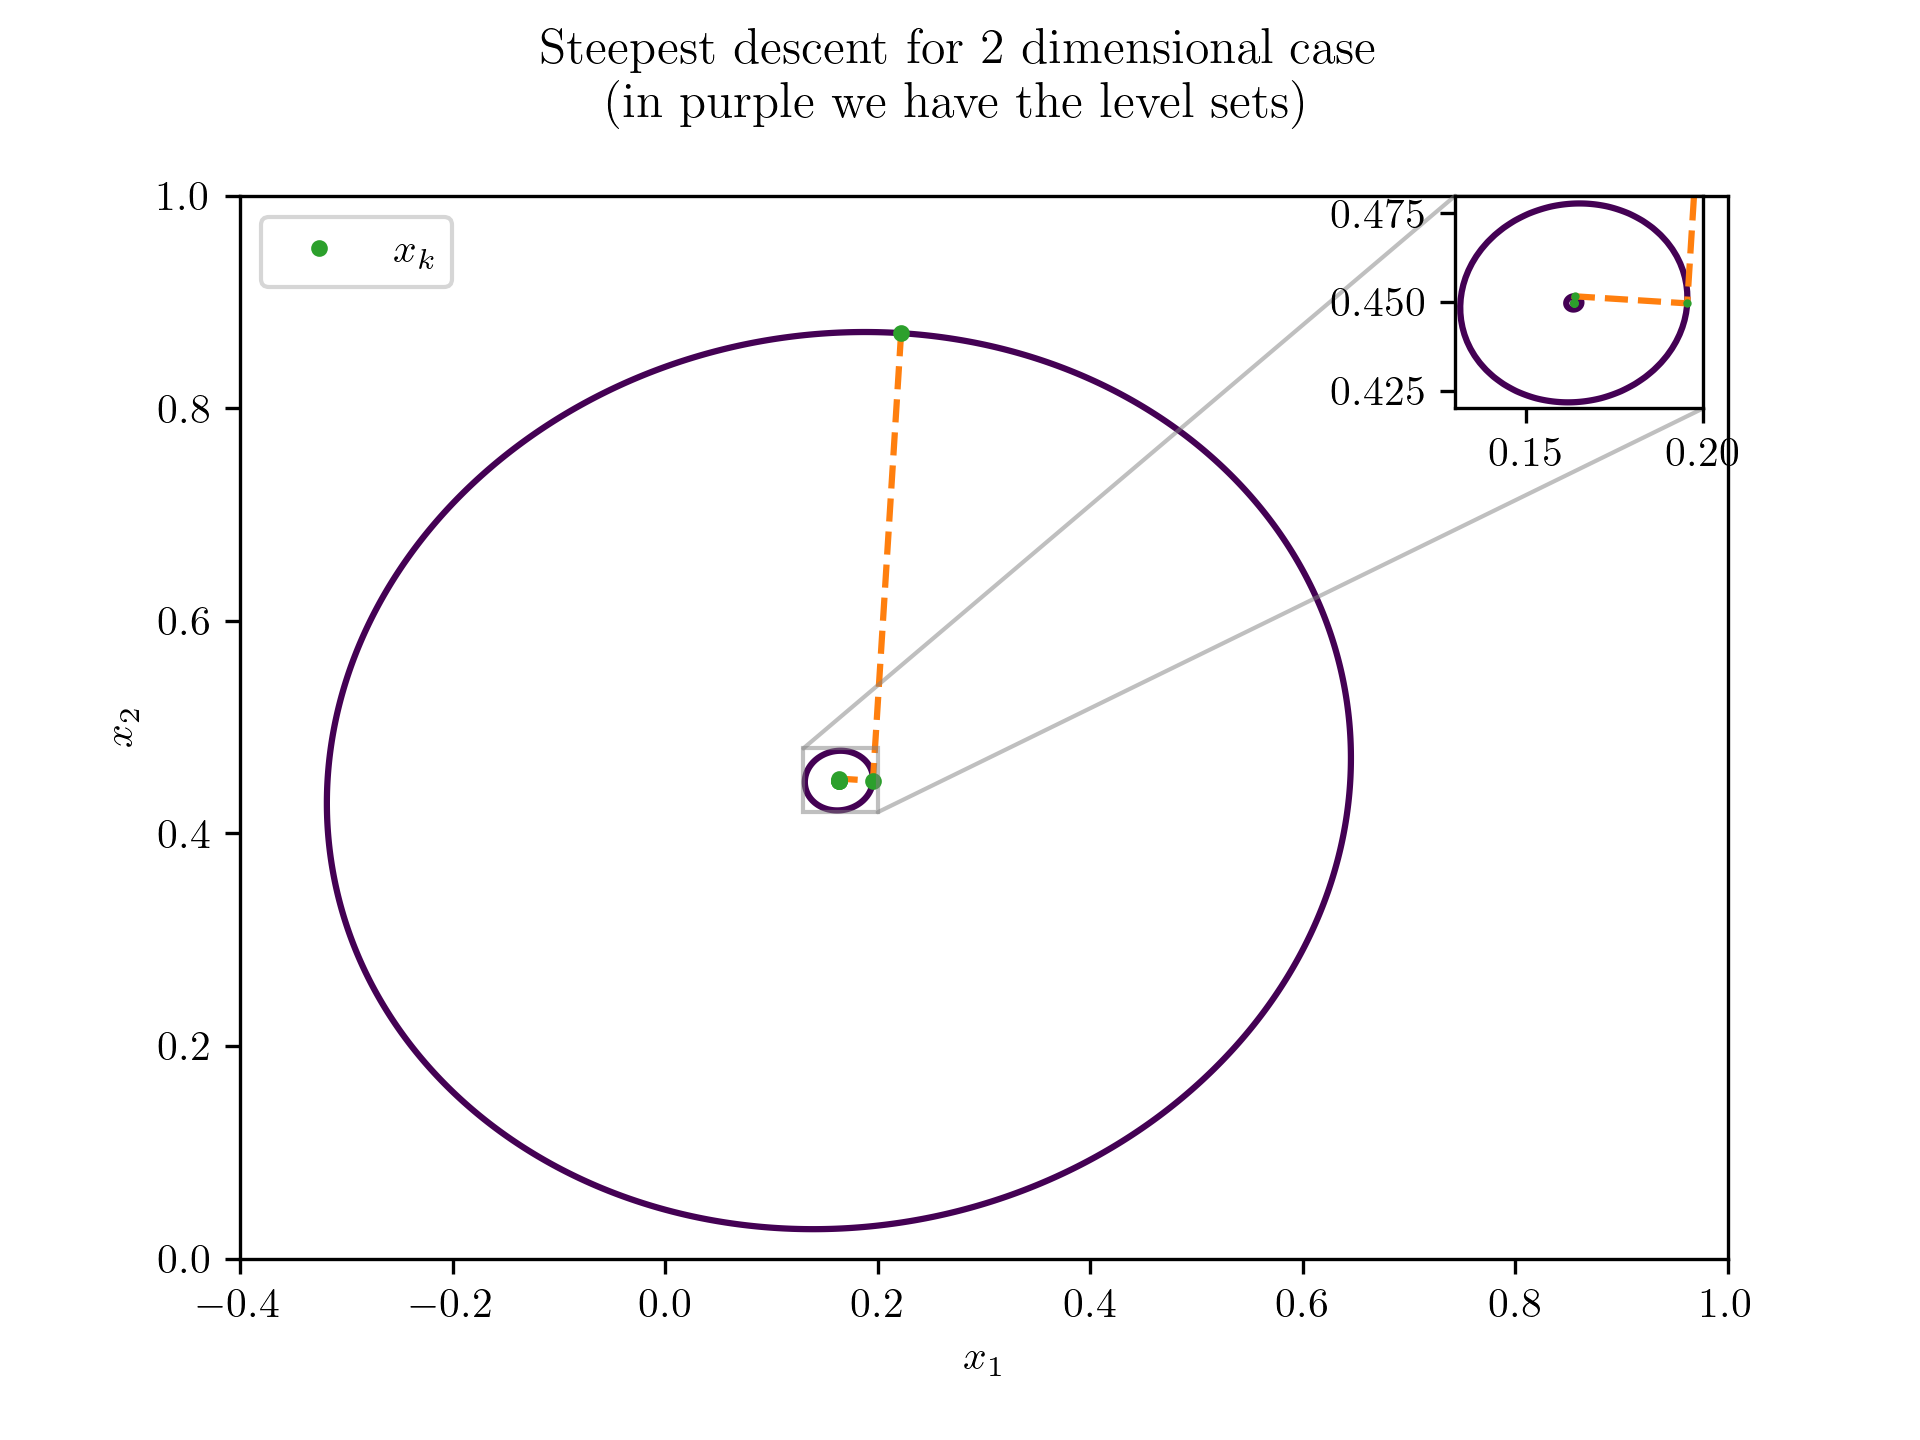
\includegraphics[width=\textwidth]{./contour_plot_1.png}
    \caption{Movement of $x^k$ towards the optimum value\label{fig:contour_sd}}
\end{figure}
I then ran this code for $n\in\{2,\dotsc,100\}$ and plotted the number of iterations
it takes for the method to converge (figure~\ref{fig:niter}). The number fluctuates
a lot (because each problem is different), but it sometimes takes steepest descent
more than 6000 steps to converge where Newton's method would have taken just 2.\par
I also plot the distribution of the number of iterations it takes steepest descent
to converge for $n=30$ from 500 runs of SD.\par
I then run the steepest descent algorithm for different $n$ but keep the condition
number fixed (and $=1000$ which is very large), we see that ill conditioning results
in increase of iterations (fig~\ref{fig:condition}).\par
Naturally, I also ran the algorithm for varying values of $n$ when the condition
number is good. See figure~\ref{fig:good}. The number of iterations are less by
a factor of 1000.\par
\begin{figure}[!htbp]
    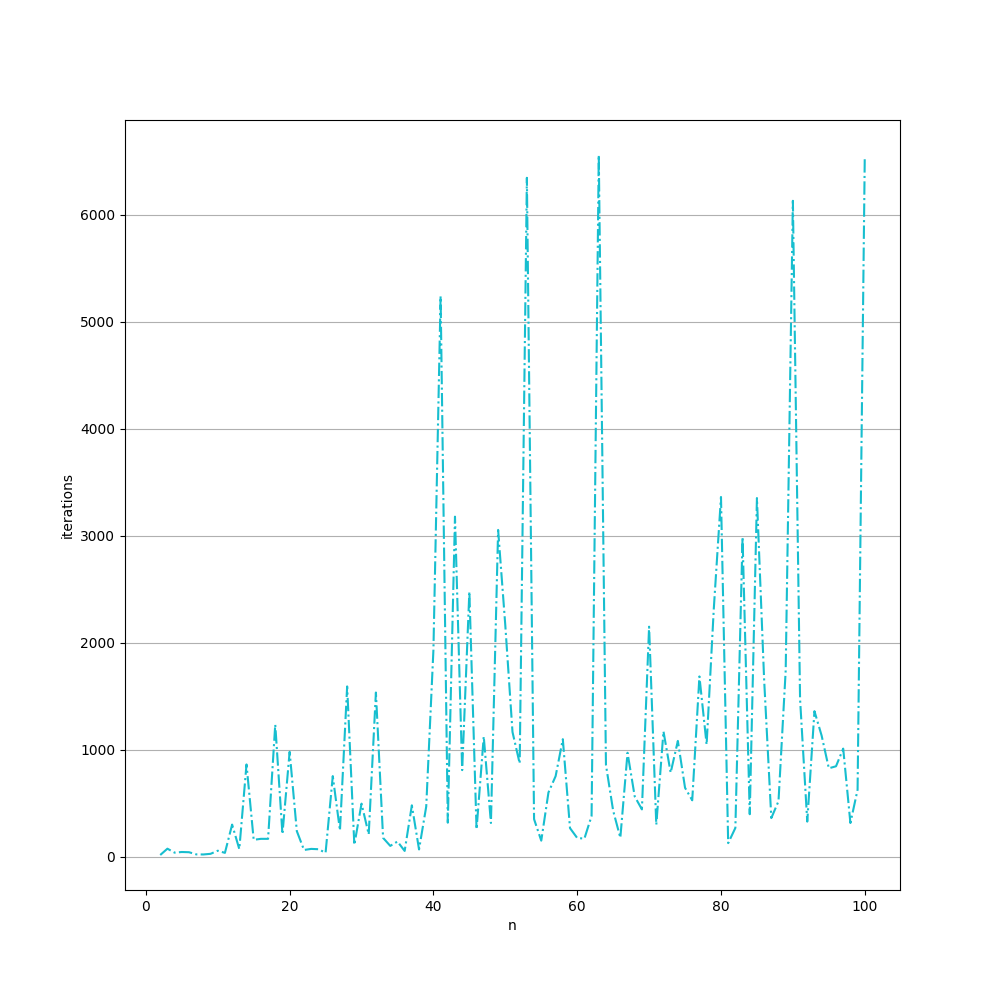
\includegraphics[width=\textwidth]{./niter.png}
    \caption{Number of iterations for convergence with varying values of $n$\label{fig:niter}}
\end{figure}
\begin{figure}[!htbp]
    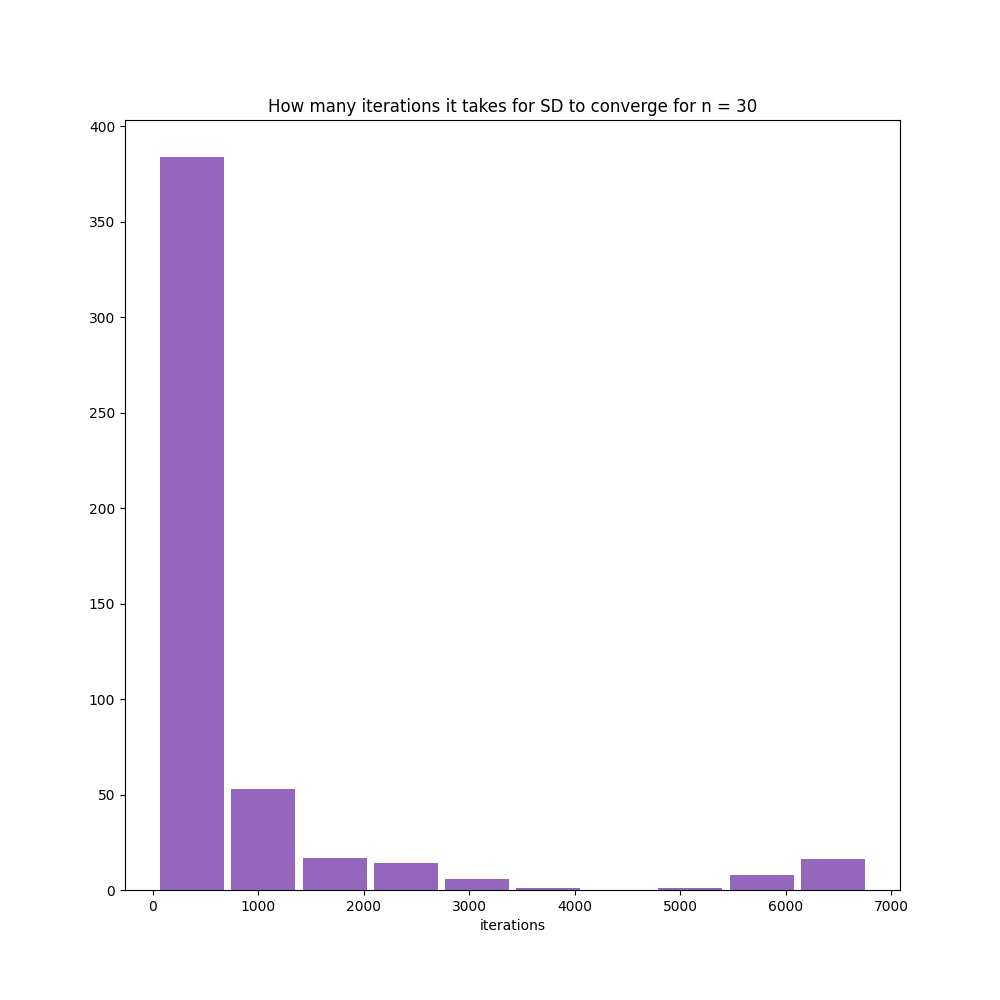
\includegraphics[width=\textwidth]{./niter_fix_n_30.png}
    \caption{Number of iteration distribution for $n=30$\label{fig:niter_30}}
\end{figure}
\begin{figure}[!htbp]
    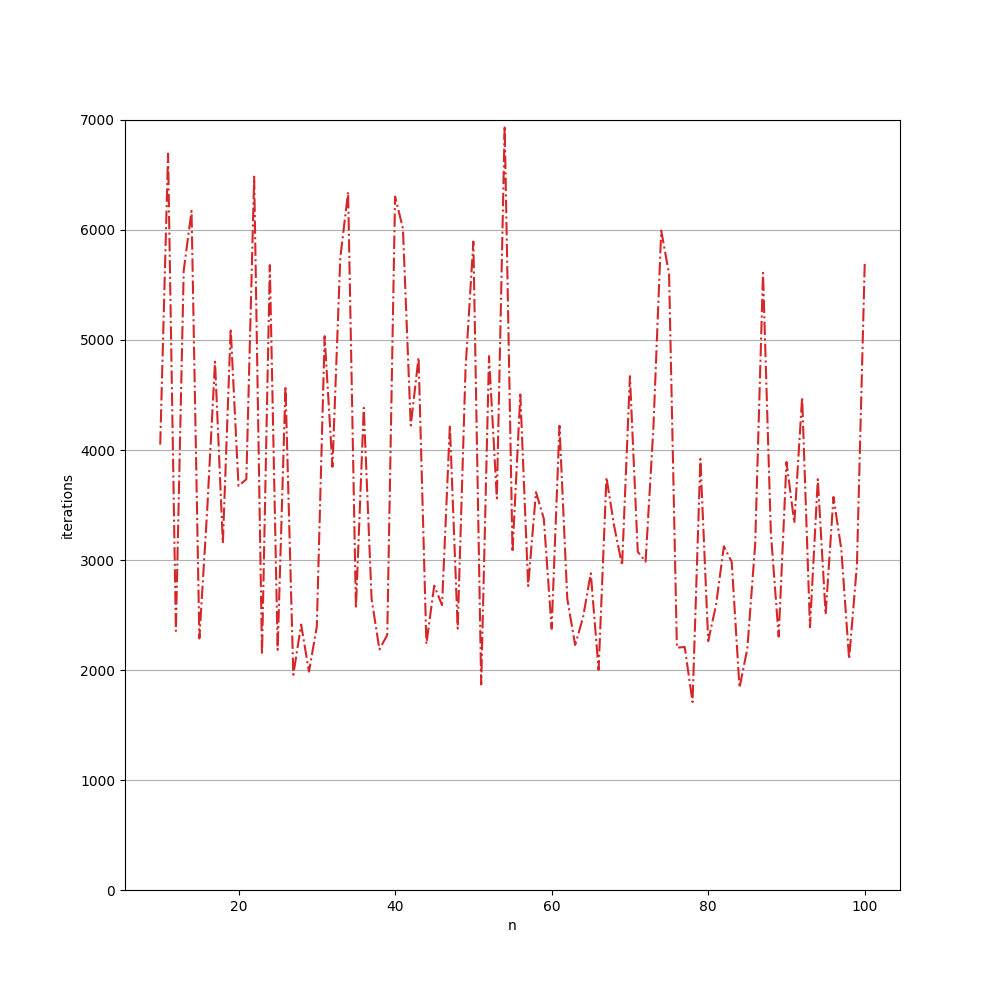
\includegraphics[width=\textwidth]{./niter_fix_r.png}
    \caption{Number of iterations for convergence with varying values of $n$
    with a fixed value of condition number $r=1000$\label{fig:condition}}
\end{figure}
\begin{figure}[!htbp]
    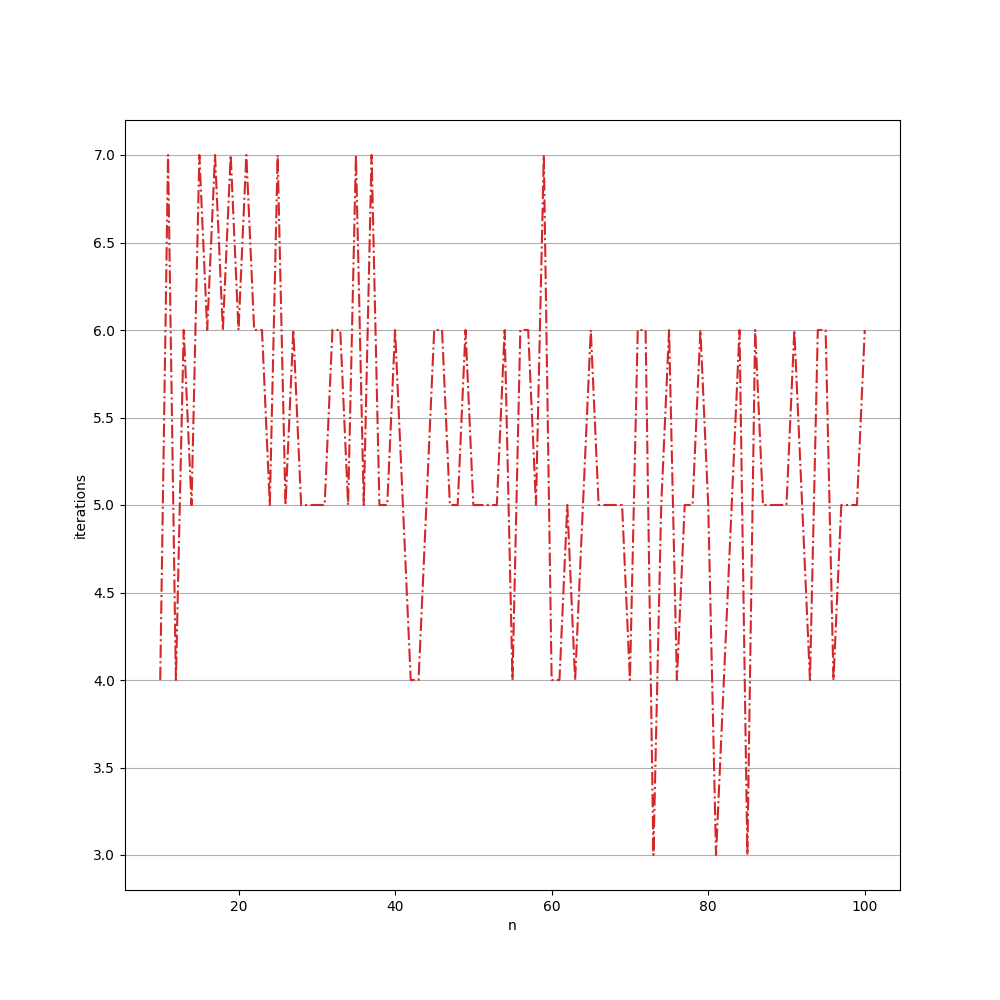
\includegraphics[width=\textwidth]{./niter_fix_r_good.png}
    \caption{Number of iterations for convergence with varying values of $n$
    with a fixed value of condition number $r=1.2$\label{fig:good}}
\end{figure}
Figure~\ref{fig:fv} shows how the function value evolves with each iteration.
We can see that the function value drops quickly in the first few iterations but
the progress quickly gets stagnant. The function value almost stays around the same
region for thousands of iterations before convergence (and note, the converged
value is still not exact.)
\begin{figure}[!htbp]
    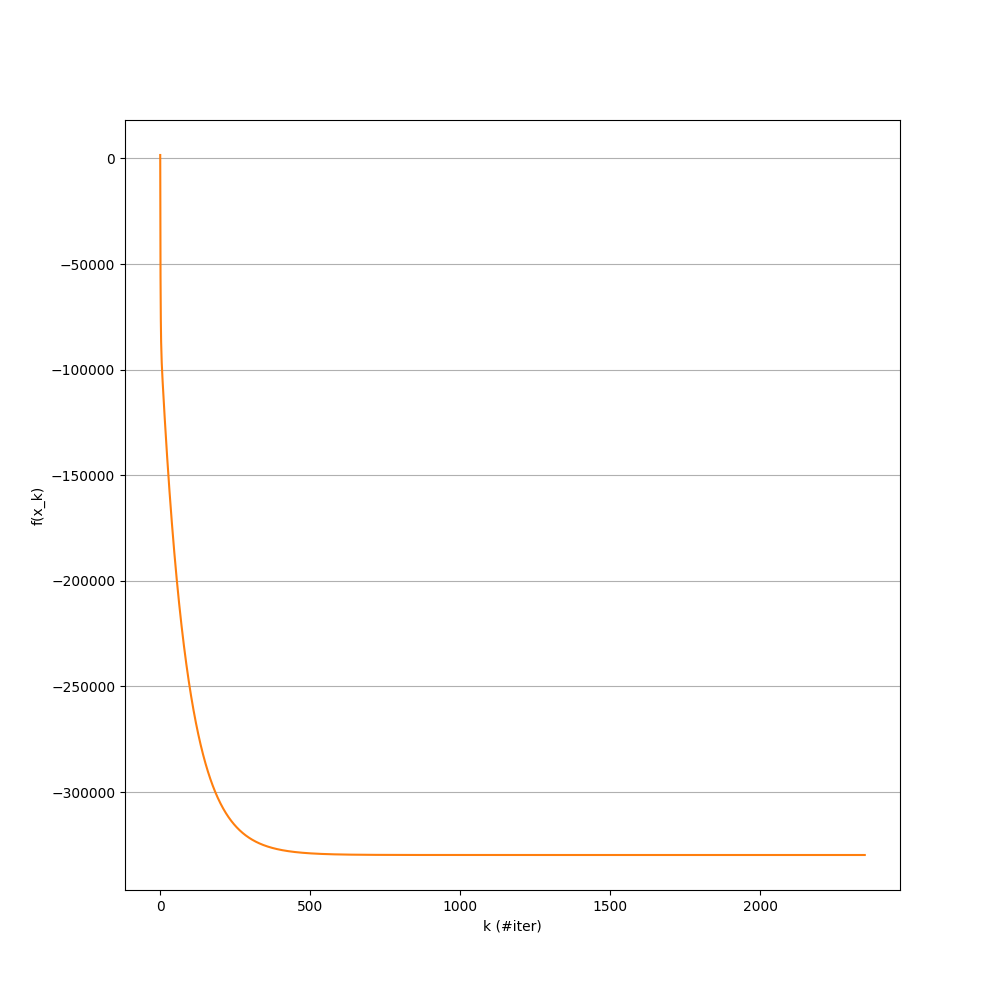
\includegraphics[width=\textwidth]{./function_value.png}
    \caption{Evolution of the function value with each successive iteration\label{fig:fv}}
\end{figure}


\section{Steepest descent for general convex functions}
I've implemented steepest descent algorithm for a general convex function. I've
outsourced gradient calculation to Harvard's \verb|autograd| library%
\footnote[1]{\url{https://github.com/HIPS/autograd}}. I've implemented
a few of the benchmark functions from the provided list, these functions reside
in the \verb|functions.py| file. The code can be run as:
\begin{verbatim}
$ python3 general_sd.py -list -function <function-name> -n <dim> -eps 1e-3 -seed 0 -alpha_hat 1e-3
\end{verbatim}
Parameters:
\begin{itemize}
    \item \verb|list|: list the implemented benchmark functions
    \item \verb|function|: benchmark function's name on which steepest descent will be run
    \item \verb|n|: the $n$ in $\mathbb{R}^n\ni x$
    \item \verb|eps|: the $\varepsilon$ used in stopping condition $\nabla f(x)<\varepsilon$
    \item \verb|seed|: same as described previously
    \item \verb|alpha_hat|: starting estimate of $\hat{\alpha}$
\end{itemize}
% Beale minimum value = 0 (so in graph too), doesn't converge by eps standards (multimodal)
% Booth minima = 0 (so in graph too), converges (plate shaped)
% Bukin n6, many local minima, global minima at 0. algo fails to converge
% Drop wave, many local minima, global minima at -1. algo converges to local minima
% sphere, converges to global minima = 0.
\begin{figure}
    \subfloat[Minimum value = 0, function is multimodal]{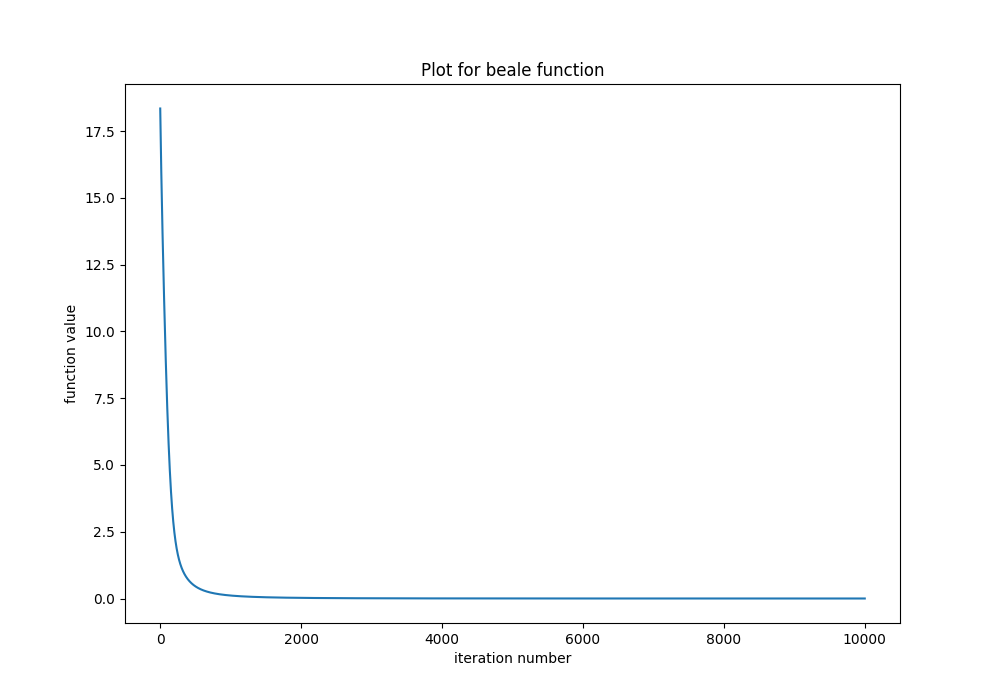
\includegraphics[width=.5\linewidth]{./SD_on_beale.png}}
    \subfloat[Minimum value = 0, function has many local minima]{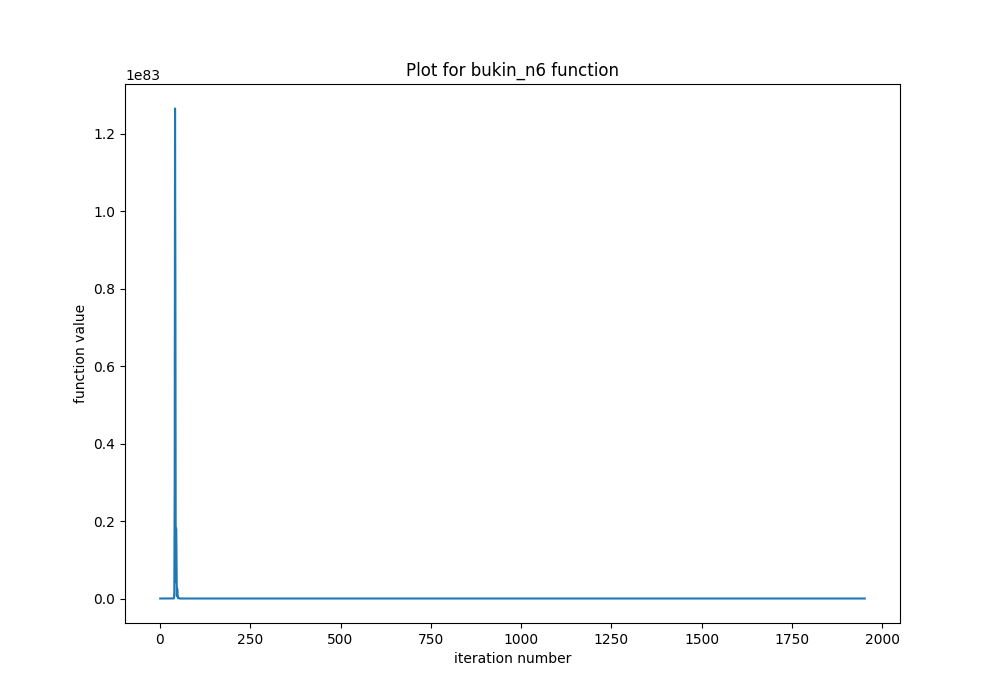
\includegraphics[width=.5\linewidth]{./SD_on_bukin_n6.png}}
    \caption{These fail to converge: in (a) the $\nabla f(x)\ge \varepsilon$ but empirically 
    $f(x)\approx 0$ while (b) just completely fails}
\end{figure}
\begin{figure}
    \subfloat[Converges to local minima]{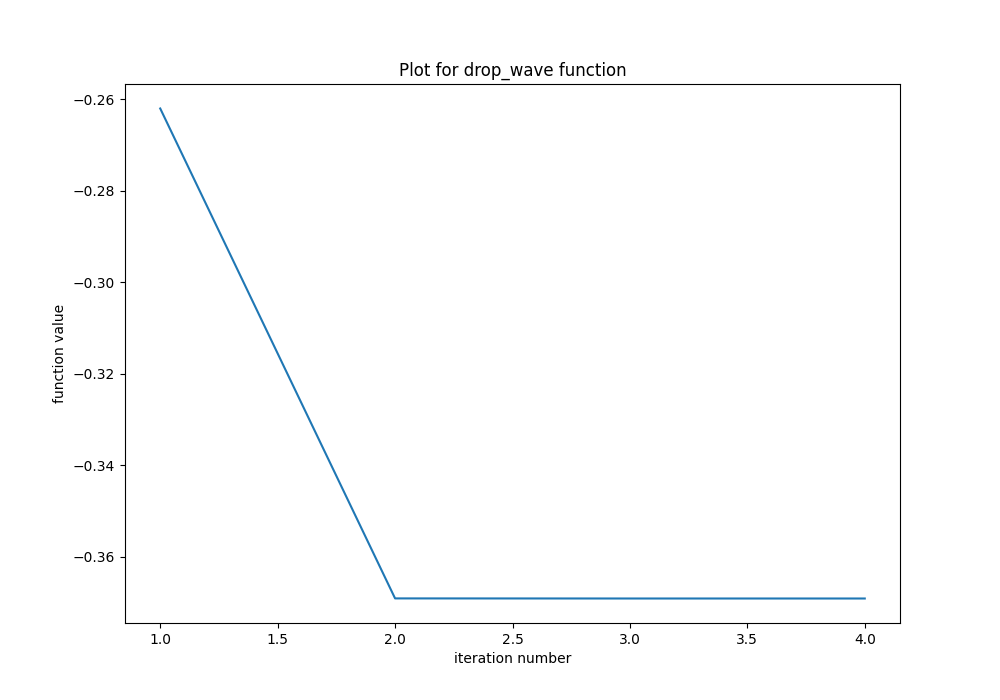
\includegraphics[width=.5\linewidth]{./SD_on_drop_wave.png}}
    \subfloat[Converges to local minima, but the function curve is very interesting]{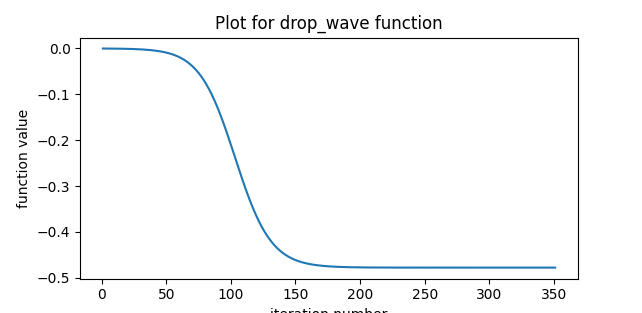
\includegraphics[width=.5\linewidth]{./drop_wave_2.png}}\\
    \subfloat[Converges to global minima]{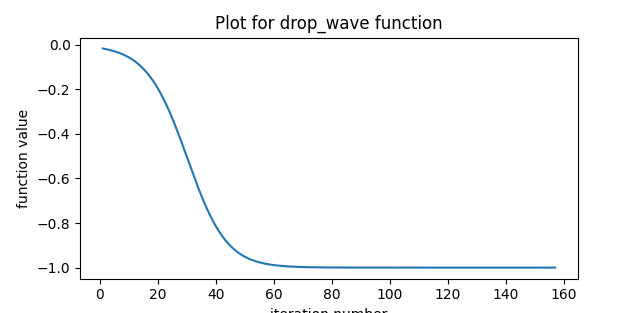
\includegraphics[width=\linewidth]{./drop_wave_3.png}}
    \caption{Global minima at 0, function has many local minima.}
\end{figure}
\begin{figure}
    \subfloat[Minimum value = 0, function is plate shaped]{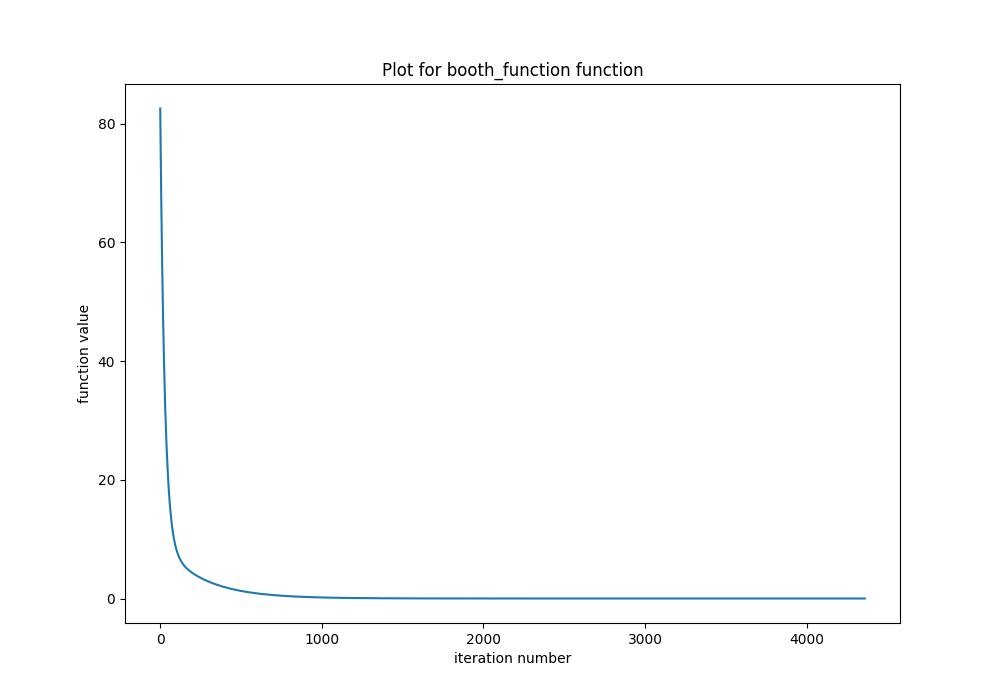
\includegraphics[width=.5\linewidth]{./SD_on_booth_function.png}}
    \subfloat[Minimum value = 0]{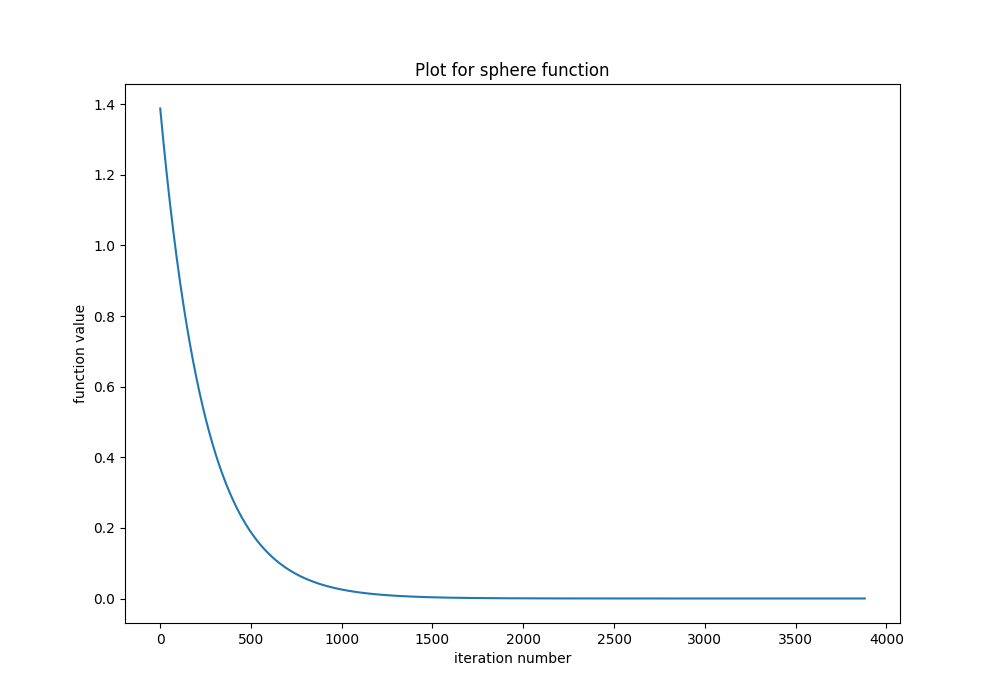
\includegraphics[width=.5\linewidth]{./SD_on_sphere.png}}
    \caption{Convergence in well behaved functions}
\end{figure}
\end{document}
